% Options for packages loaded elsewhere
\PassOptionsToPackage{unicode}{hyperref}
\PassOptionsToPackage{hyphens}{url}
%
\documentclass[
]{article}
\usepackage{amsmath,amssymb}
\usepackage{lmodern}
\usepackage{ifxetex,ifluatex}
\ifnum 0\ifxetex 1\fi\ifluatex 1\fi=0 % if pdftex
  \usepackage[T1]{fontenc}
  \usepackage[utf8]{inputenc}
  \usepackage{textcomp} % provide euro and other symbols
\else % if luatex or xetex
  \usepackage{unicode-math}
  \defaultfontfeatures{Scale=MatchLowercase}
  \defaultfontfeatures[\rmfamily]{Ligatures=TeX,Scale=1}
\fi
% Use upquote if available, for straight quotes in verbatim environments
\IfFileExists{upquote.sty}{\usepackage{upquote}}{}
\IfFileExists{microtype.sty}{% use microtype if available
  \usepackage[]{microtype}
  \UseMicrotypeSet[protrusion]{basicmath} % disable protrusion for tt fonts
}{}
\makeatletter
\@ifundefined{KOMAClassName}{% if non-KOMA class
  \IfFileExists{parskip.sty}{%
    \usepackage{parskip}
  }{% else
    \setlength{\parindent}{0pt}
    \setlength{\parskip}{6pt plus 2pt minus 1pt}}
}{% if KOMA class
  \KOMAoptions{parskip=half}}
\makeatother
\usepackage{xcolor}
\IfFileExists{xurl.sty}{\usepackage{xurl}}{} % add URL line breaks if available
\IfFileExists{bookmark.sty}{\usepackage{bookmark}}{\usepackage{hyperref}}
\hypersetup{
  pdftitle={IO \& Econometrics workshop - PS1},
  pdfauthor={Doron Zamir},
  hidelinks,
  pdfcreator={LaTeX via pandoc}}
\urlstyle{same} % disable monospaced font for URLs
\usepackage[margin=1in]{geometry}
\usepackage{color}
\usepackage{fancyvrb}
\newcommand{\VerbBar}{|}
\newcommand{\VERB}{\Verb[commandchars=\\\{\}]}
\DefineVerbatimEnvironment{Highlighting}{Verbatim}{commandchars=\\\{\}}
% Add ',fontsize=\small' for more characters per line
\usepackage{framed}
\definecolor{shadecolor}{RGB}{248,248,248}
\newenvironment{Shaded}{\begin{snugshade}}{\end{snugshade}}
\newcommand{\AlertTok}[1]{\textcolor[rgb]{0.94,0.16,0.16}{#1}}
\newcommand{\AnnotationTok}[1]{\textcolor[rgb]{0.56,0.35,0.01}{\textbf{\textit{#1}}}}
\newcommand{\AttributeTok}[1]{\textcolor[rgb]{0.77,0.63,0.00}{#1}}
\newcommand{\BaseNTok}[1]{\textcolor[rgb]{0.00,0.00,0.81}{#1}}
\newcommand{\BuiltInTok}[1]{#1}
\newcommand{\CharTok}[1]{\textcolor[rgb]{0.31,0.60,0.02}{#1}}
\newcommand{\CommentTok}[1]{\textcolor[rgb]{0.56,0.35,0.01}{\textit{#1}}}
\newcommand{\CommentVarTok}[1]{\textcolor[rgb]{0.56,0.35,0.01}{\textbf{\textit{#1}}}}
\newcommand{\ConstantTok}[1]{\textcolor[rgb]{0.00,0.00,0.00}{#1}}
\newcommand{\ControlFlowTok}[1]{\textcolor[rgb]{0.13,0.29,0.53}{\textbf{#1}}}
\newcommand{\DataTypeTok}[1]{\textcolor[rgb]{0.13,0.29,0.53}{#1}}
\newcommand{\DecValTok}[1]{\textcolor[rgb]{0.00,0.00,0.81}{#1}}
\newcommand{\DocumentationTok}[1]{\textcolor[rgb]{0.56,0.35,0.01}{\textbf{\textit{#1}}}}
\newcommand{\ErrorTok}[1]{\textcolor[rgb]{0.64,0.00,0.00}{\textbf{#1}}}
\newcommand{\ExtensionTok}[1]{#1}
\newcommand{\FloatTok}[1]{\textcolor[rgb]{0.00,0.00,0.81}{#1}}
\newcommand{\FunctionTok}[1]{\textcolor[rgb]{0.00,0.00,0.00}{#1}}
\newcommand{\ImportTok}[1]{#1}
\newcommand{\InformationTok}[1]{\textcolor[rgb]{0.56,0.35,0.01}{\textbf{\textit{#1}}}}
\newcommand{\KeywordTok}[1]{\textcolor[rgb]{0.13,0.29,0.53}{\textbf{#1}}}
\newcommand{\NormalTok}[1]{#1}
\newcommand{\OperatorTok}[1]{\textcolor[rgb]{0.81,0.36,0.00}{\textbf{#1}}}
\newcommand{\OtherTok}[1]{\textcolor[rgb]{0.56,0.35,0.01}{#1}}
\newcommand{\PreprocessorTok}[1]{\textcolor[rgb]{0.56,0.35,0.01}{\textit{#1}}}
\newcommand{\RegionMarkerTok}[1]{#1}
\newcommand{\SpecialCharTok}[1]{\textcolor[rgb]{0.00,0.00,0.00}{#1}}
\newcommand{\SpecialStringTok}[1]{\textcolor[rgb]{0.31,0.60,0.02}{#1}}
\newcommand{\StringTok}[1]{\textcolor[rgb]{0.31,0.60,0.02}{#1}}
\newcommand{\VariableTok}[1]{\textcolor[rgb]{0.00,0.00,0.00}{#1}}
\newcommand{\VerbatimStringTok}[1]{\textcolor[rgb]{0.31,0.60,0.02}{#1}}
\newcommand{\WarningTok}[1]{\textcolor[rgb]{0.56,0.35,0.01}{\textbf{\textit{#1}}}}
\usepackage{longtable,booktabs,array}
\usepackage{calc} % for calculating minipage widths
% Correct order of tables after \paragraph or \subparagraph
\usepackage{etoolbox}
\makeatletter
\patchcmd\longtable{\par}{\if@noskipsec\mbox{}\fi\par}{}{}
\makeatother
% Allow footnotes in longtable head/foot
\IfFileExists{footnotehyper.sty}{\usepackage{footnotehyper}}{\usepackage{footnote}}
\makesavenoteenv{longtable}
\usepackage{graphicx}
\makeatletter
\def\maxwidth{\ifdim\Gin@nat@width>\linewidth\linewidth\else\Gin@nat@width\fi}
\def\maxheight{\ifdim\Gin@nat@height>\textheight\textheight\else\Gin@nat@height\fi}
\makeatother
% Scale images if necessary, so that they will not overflow the page
% margins by default, and it is still possible to overwrite the defaults
% using explicit options in \includegraphics[width, height, ...]{}
\setkeys{Gin}{width=\maxwidth,height=\maxheight,keepaspectratio}
% Set default figure placement to htbp
\makeatletter
\def\fps@figure{htbp}
\makeatother
\setlength{\emergencystretch}{3em} % prevent overfull lines
\providecommand{\tightlist}{%
  \setlength{\itemsep}{0pt}\setlength{\parskip}{0pt}}
\setcounter{secnumdepth}{-\maxdimen} % remove section numbering
\ifluatex
  \usepackage{selnolig}  % disable illegal ligatures
\fi

\title{IO \& Econometrics workshop - PS1}
\author{Doron Zamir}
\date{}

\begin{document}
\maketitle

This is a markdown file created using RStudio.

\hypertarget{using-packeges}{%
\subsubsection{Using Packeges}\label{using-packeges}}

I used these packages to create the data:

\begin{Shaded}
\begin{Highlighting}[]
\FunctionTok{library}\NormalTok{(tidyverse)}
\FunctionTok{library}\NormalTok{(knitr)}
\FunctionTok{library}\NormalTok{(magrittr)}
\FunctionTok{library}\NormalTok{(AER)}
\FunctionTok{library}\NormalTok{(broom)}
\end{Highlighting}
\end{Shaded}

\hypertarget{tidy-the-data}{%
\subsection{Tidy the Data}\label{tidy-the-data}}

\hypertarget{importing-data}{%
\subsubsection{Importing Data}\label{importing-data}}

I used the data from
\href{https://davidcard.berkeley.edu/data_sets.html}{David Card's
website} The relevant file is \texttt{nls.dat} saved in the
\texttt{Data} directory.

\begin{Shaded}
\begin{Highlighting}[]
\NormalTok{data }\OtherTok{\textless{}{-}} \FunctionTok{read.table}\NormalTok{(}\StringTok{"Data/nls.dat"}\NormalTok{) }\SpecialCharTok{\%\textgreater{}\%} \FunctionTok{as\_data\_frame}\NormalTok{()}
\FunctionTok{head}\NormalTok{(data)}
\end{Highlighting}
\end{Shaded}

\begin{verbatim}
## # A tibble: 6 x 52
##      V1    V2    V3    V4    V5    V6    V7    V8    V9   V10   V11   V12    V13
##   <int> <int> <int> <int> <int> <int> <int> <int> <dbl> <int> <dbl> <int>  <int>
## 1     2     0     0     0     0     7     5    29  9.94     1  10.2     1 158413
## 2     3     0     0     0     0    12    11    27  8        0   8       0 380166
## 3     4     0     0     0     0    12    12    34 14        0  12       0 367470
## 4     5     1     1     1     0    11    11    27 11        0  12       0 380166
## 5     6     1     1     1     0    12    12    34  8        0   7       0 367470
## 6     7     1     1     1     0    12    11    26  9        0  12       0 380166
## # ... with 39 more variables: V14 <int>, V15 <int>, V16 <int>, V17 <int>,
## #   V18 <int>, V19 <int>, V20 <int>, V21 <int>, V22 <int>, V23 <int>,
## #   V24 <int>, V25 <int>, V26 <int>, V27 <int>, V28 <int>, V29 <chr>,
## #   V30 <chr>, V31 <int>, V32 <int>, V33 <int>, V34 <chr>, V35 <int>,
## #   V36 <chr>, V37 <chr>, V38 <int>, V39 <chr>, V40 <chr>, V41 <chr>,
## #   V42 <int>, V43 <int>, V44 <int>, V45 <chr>, V46 <chr>, V47 <chr>,
## #   V48 <chr>, V49 <chr>, V50 <chr>, V51 <chr>, V52 <chr>
\end{verbatim}

\hypertarget{changing-col-names-type}{%
\subsubsection{Changing col names \&
type}\label{changing-col-names-type}}

Using variable names from `code\_bk.txt'

\begin{Shaded}
\begin{Highlighting}[]
\FunctionTok{colnames}\NormalTok{(data) }\OtherTok{\textless{}{-}}\NormalTok{(}\FunctionTok{c}\NormalTok{(}\StringTok{"id"}\NormalTok{,}\StringTok{"nearc2"}\NormalTok{,}\StringTok{"nearc4"}\NormalTok{,}\StringTok{"nearc4a"}\NormalTok{,}\StringTok{"nearc4b"}\NormalTok{,}\StringTok{"ed76"}\NormalTok{,}\StringTok{"ed66"}\NormalTok{,}\StringTok{"age76"}\NormalTok{,}\StringTok{"daded"}\NormalTok{,}\StringTok{"nodaded"}\NormalTok{,}\StringTok{"momed"}\NormalTok{,}\StringTok{"nomomed"}\NormalTok{,}\StringTok{"weight"}\NormalTok{,}\StringTok{"momdad14"}\NormalTok{,}\StringTok{"sinmom14"}\NormalTok{,}\StringTok{"step14"}\NormalTok{,}\StringTok{"reg661"}\NormalTok{,}\StringTok{"reg662"}\NormalTok{,}\StringTok{"reg663"}\NormalTok{,}\StringTok{"reg664"}\NormalTok{,}\StringTok{"reg665"}\NormalTok{,}\StringTok{"reg666"}\NormalTok{,}\StringTok{"reg667"}\NormalTok{,}\StringTok{"reg668"}\NormalTok{,}\StringTok{"reg669"}\NormalTok{,}\StringTok{"south66"}\NormalTok{,}\StringTok{"work76"}\NormalTok{,}\StringTok{"work78"}\NormalTok{,}\StringTok{"lwage76"}\NormalTok{,}\StringTok{"lwage78"}\NormalTok{,}\StringTok{"famed"}\NormalTok{,}\StringTok{"black"}\NormalTok{,}\StringTok{"smsa76r"}\NormalTok{,}\StringTok{"smsa78r"}\NormalTok{,}\StringTok{"reg76r"}\NormalTok{,}\StringTok{"reg78r"}\NormalTok{,}\StringTok{"reg80r"}\NormalTok{,}\StringTok{"smsa66r"}\NormalTok{,}\StringTok{"wage76"}\NormalTok{,}\StringTok{"wage78"}\NormalTok{,}\StringTok{"wage80"}\NormalTok{,}\StringTok{"noint78"}\NormalTok{,}\StringTok{"noint80"}\NormalTok{,}\StringTok{"enroll76"}\NormalTok{,}\StringTok{"enroll78"}\NormalTok{,}\StringTok{"enroll80"}\NormalTok{,}\StringTok{"kww"}\NormalTok{,}\StringTok{"iq"}\NormalTok{,}\StringTok{"marsta76"}\NormalTok{,}\StringTok{"marsta78"}\NormalTok{,}\StringTok{"marsta80"}\NormalTok{,}\StringTok{"libcrd14"}\NormalTok{))}

\NormalTok{data }\SpecialCharTok{\%\textless{}\textgreater{}\%} \FunctionTok{mutate\_if}\NormalTok{(is\_character,}\FunctionTok{suppressWarnings}\NormalTok{(as.numeric))}
\FunctionTok{head}\NormalTok{(data)}
\end{Highlighting}
\end{Shaded}

\begin{verbatim}
## # A tibble: 6 x 52
##      id nearc2 nearc4 nearc4a nearc4b  ed76  ed66 age76 daded nodaded momed
##   <int>  <int>  <int>   <int>   <int> <int> <int> <int> <dbl>   <int> <dbl>
## 1     2      0      0       0       0     7     5    29  9.94       1  10.2
## 2     3      0      0       0       0    12    11    27  8          0   8  
## 3     4      0      0       0       0    12    12    34 14          0  12  
## 4     5      1      1       1       0    11    11    27 11          0  12  
## 5     6      1      1       1       0    12    12    34  8          0   7  
## 6     7      1      1       1       0    12    11    26  9          0  12  
## # ... with 41 more variables: nomomed <int>, weight <int>, momdad14 <int>,
## #   sinmom14 <int>, step14 <int>, reg661 <int>, reg662 <int>, reg663 <int>,
## #   reg664 <int>, reg665 <int>, reg666 <int>, reg667 <int>, reg668 <int>,
## #   reg669 <int>, south66 <int>, work76 <int>, work78 <int>, lwage76 <dbl>,
## #   lwage78 <dbl>, famed <int>, black <int>, smsa76r <int>, smsa78r <dbl>,
## #   reg76r <int>, reg78r <dbl>, reg80r <dbl>, smsa66r <int>, wage76 <dbl>,
## #   wage78 <dbl>, wage80 <dbl>, noint78 <int>, noint80 <int>, enroll76 <int>,
## #   enroll78 <dbl>, enroll80 <dbl>, kww <dbl>, iq <dbl>, marsta76 <dbl>,
## #   marsta78 <dbl>, marsta80 <dbl>, libcrd14 <dbl>
\end{verbatim}

\hypertarget{creating-new-varibales-for-experiance}{%
\subsubsection{Creating new Varibales for
experiance}\label{creating-new-varibales-for-experiance}}

\[exp76=age76-ed76-6\] \[exp762=exp76*exp76\]

\begin{Shaded}
\begin{Highlighting}[]
\NormalTok{data }\OtherTok{\textless{}{-}}\NormalTok{ data }\SpecialCharTok{\%\textgreater{}\%} \FunctionTok{mutate}\NormalTok{(}\AttributeTok{exp76 =}\NormalTok{  age76}\SpecialCharTok{{-}}\NormalTok{ed76 }\SpecialCharTok{{-}} \DecValTok{6}\NormalTok{)}
\NormalTok{data }\OtherTok{\textless{}{-}}\NormalTok{ data }\SpecialCharTok{\%\textgreater{}\%} \FunctionTok{mutate}\NormalTok{(}\AttributeTok{exp762 =}\NormalTok{ exp76 }\SpecialCharTok{**} \DecValTok{2}\NormalTok{)}
\end{Highlighting}
\end{Shaded}

\hypertarget{sumaarise-data}{%
\subsubsection{Sumaarise Data}\label{sumaarise-data}}

\begin{Shaded}
\begin{Highlighting}[]
\NormalTok{data\_summary }\OtherTok{\textless{}{-}}\NormalTok{ data[}\SpecialCharTok{{-}}\DecValTok{1}\NormalTok{] }\SpecialCharTok{\%\textgreater{}\%}
  \FunctionTok{summarise\_all}\NormalTok{(}\FunctionTok{list}\NormalTok{(}
    \AttributeTok{Min =}\NormalTok{ min, }
    \AttributeTok{Mean =}\NormalTok{ mean, }
    \AttributeTok{Max =}\NormalTok{ max,}
    \AttributeTok{SD =}\NormalTok{ sd)) }\SpecialCharTok{\%\textgreater{}\%}
  \FunctionTok{pivot\_longer}\NormalTok{(}\FunctionTok{everything}\NormalTok{(),}
               \AttributeTok{names\_to =} \FunctionTok{c}\NormalTok{(}\StringTok{"Var"}\NormalTok{,}\StringTok{"Stat"}\NormalTok{),}
               \AttributeTok{names\_sep =} \StringTok{"\_"}\NormalTok{) }\SpecialCharTok{\%\textgreater{}\%}
  \FunctionTok{pivot\_wider}\NormalTok{(}\AttributeTok{names\_from =} \StringTok{"Stat"}\NormalTok{) }\SpecialCharTok{\%\textgreater{}\%} \FunctionTok{column\_to\_rownames}\NormalTok{(}\StringTok{"Var"}\NormalTok{) }
\NormalTok{data\_summary }\SpecialCharTok{\%\textgreater{}\%} \FunctionTok{format}\NormalTok{(}\AttributeTok{scientific =} \ConstantTok{FALSE}\NormalTok{, }\AttributeTok{digits =} \DecValTok{2}\NormalTok{,}\AttributeTok{trim =} \ConstantTok{TRUE}\NormalTok{)  }
\end{Highlighting}
\end{Shaded}

\begin{verbatim}
##            Min       Mean     Max        SD
## nearc2       0      0.432       1      0.50
## nearc4       0      0.678       1      0.47
## nearc4a      0      0.492       1      0.50
## nearc4b      0      0.186       1      0.39
## ed76         0     13.225      18      2.75
## ed66         0     10.743      18      2.46
## age76       24     28.175      34      3.17
## daded        0     10.003      18      3.30
## nodaded      0      0.224       1      0.42
## momed        0     10.342      18      3.03
## nomomed      0      0.114       1      0.32
## weight   75607 320318.351 1752340 168006.76
## momdad14     0      0.792       1      0.41
## sinmom14     0      0.100       1      0.30
## step14       0      0.038       1      0.19
## reg661       0      0.045       1      0.21
## reg662       0      0.155       1      0.36
## reg663       0      0.194       1      0.40
## reg664       0      0.069       1      0.25
## reg665       0      0.210       1      0.41
## reg666       0      0.093       1      0.29
## reg667       0      0.110       1      0.31
## reg668       0      0.031       1      0.17
## reg669       0      0.094       1      0.29
## south66      0      0.413       1      0.49
## work76       0      0.835       1      0.37
## work78       0      0.735       1      0.44
## lwage76     NA         NA      NA        NA
## lwage78     NA         NA      NA        NA
## famed        1      5.913       9      2.65
## black        0      0.230       1      0.42
## smsa76r      0      0.695       1      0.46
## smsa78r     NA         NA      NA        NA
## reg76r       0      0.400       1      0.49
## reg78r      NA         NA      NA        NA
## reg80r      NA         NA      NA        NA
## smsa66r      0      0.643       1      0.48
## wage76      NA         NA      NA        NA
## wage78      NA         NA      NA        NA
## wage80      NA         NA      NA        NA
## noint78      0      0.081       1      0.27
## noint80      0      0.107       1      0.31
## enroll76     0      0.095       1      0.29
## enroll78    NA         NA      NA        NA
## enroll80    NA         NA      NA        NA
## kww         NA         NA      NA        NA
## iq          NA         NA      NA        NA
## marsta76    NA         NA      NA        NA
## marsta78    NA         NA      NA        NA
## marsta80    NA         NA      NA        NA
## libcrd14    NA         NA      NA        NA
## exp76        0      8.950      25      4.22
## exp762       0     97.868     625     87.89
\end{verbatim}

\#\#plotting some of it

\begin{Shaded}
\begin{Highlighting}[]
\NormalTok{data\_to\_plot }\OtherTok{\textless{}{-}}\NormalTok{ data }\SpecialCharTok{\%\textgreater{}\%} 
  \FunctionTok{mutate}\NormalTok{(}
    \AttributeTok{black =} \FunctionTok{factor}\NormalTok{(black,}\AttributeTok{labels =} \FunctionTok{c}\NormalTok{(}\StringTok{"no"}\NormalTok{,}\StringTok{"yes"}\NormalTok{)),}
    \AttributeTok{nearc4=}\FunctionTok{factor}\NormalTok{(nearc4,}\AttributeTok{labels =} \FunctionTok{c}\NormalTok{(}\StringTok{"no"}\NormalTok{,}\StringTok{"yes"}\NormalTok{)),}
\NormalTok{         )}
\end{Highlighting}
\end{Shaded}

\hypertarget{education-and-lwage}{%
\subsubsection{education and lwage}\label{education-and-lwage}}

\begin{Shaded}
\begin{Highlighting}[]
\NormalTok{data\_to\_plot }\SpecialCharTok{\%\textgreater{}\%} \FunctionTok{ggplot}\NormalTok{(}\FunctionTok{aes}\NormalTok{(ed76,lwage78)) }\SpecialCharTok{+}
  \FunctionTok{geom\_point}\NormalTok{(}\FunctionTok{aes}\NormalTok{(}
    \AttributeTok{color =}\NormalTok{ nearc4),}
    \AttributeTok{alpha =}\FloatTok{0.4}\NormalTok{ ) }\SpecialCharTok{+}
  \FunctionTok{geom\_smooth}\NormalTok{(}\AttributeTok{method =}\NormalTok{ lm)}
\end{Highlighting}
\end{Shaded}

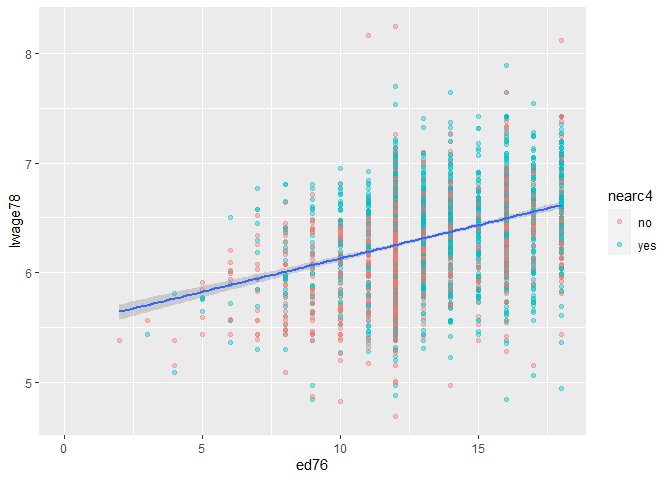
\includegraphics{ps1_iv_card_schholing_files/figure-latex/unnamed-chunk-8-1.pdf}
\#\#splitting by distance from collage

\begin{Shaded}
\begin{Highlighting}[]
\NormalTok{data\_to\_plot }\SpecialCharTok{\%\textgreater{}\%} \FunctionTok{ggplot}\NormalTok{(}\FunctionTok{aes}\NormalTok{(ed76,lwage78)) }\SpecialCharTok{+}
  \FunctionTok{geom\_point}\NormalTok{(}\FunctionTok{aes}\NormalTok{(}
    \AttributeTok{color =}\NormalTok{ black),}
    \AttributeTok{alpha =}\FloatTok{0.4}\NormalTok{ ) }\SpecialCharTok{+}
  \FunctionTok{geom\_smooth}\NormalTok{(}\AttributeTok{method =}\NormalTok{ lm)}\SpecialCharTok{+}
  \FunctionTok{facet\_grid}\NormalTok{(}\AttributeTok{cols =} \FunctionTok{vars}\NormalTok{(nearc4))}
\end{Highlighting}
\end{Shaded}

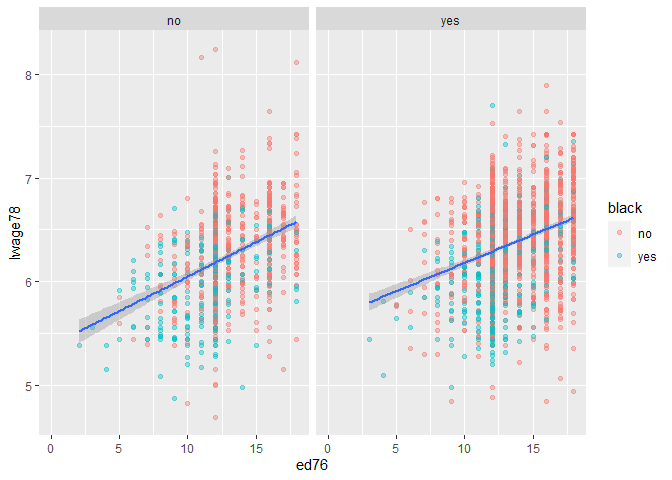
\includegraphics{ps1_iv_card_schholing_files/figure-latex/unnamed-chunk-9-1.pdf}
\#\#\# histogram of ed76

\begin{Shaded}
\begin{Highlighting}[]
\NormalTok{data\_to\_plot }\SpecialCharTok{\%\textgreater{}\%} \FunctionTok{ggplot}\NormalTok{(}\FunctionTok{aes}\NormalTok{(ed76)) }\SpecialCharTok{+} 
  \FunctionTok{geom\_bar}\NormalTok{(}\FunctionTok{aes}\NormalTok{(}
    \AttributeTok{fill =}\NormalTok{ black)) }\SpecialCharTok{+} 
  \FunctionTok{facet\_grid}\NormalTok{(}\AttributeTok{row =} \FunctionTok{vars}\NormalTok{(nearc4))}
\end{Highlighting}
\end{Shaded}

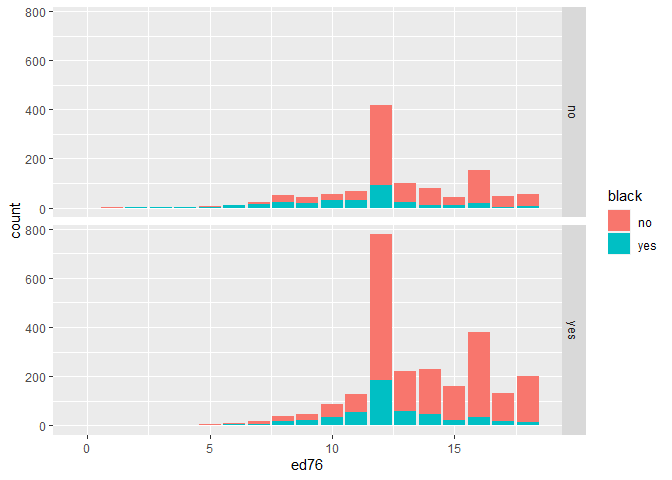
\includegraphics{ps1_iv_card_schholing_files/figure-latex/unnamed-chunk-10-1.pdf}

\hypertarget{estimating-a-model}{%
\subsection{Estimating a model}\label{estimating-a-model}}

\#\#\#OLS \[ lwage78 = \alpha \cdot ed76 + \beta \cdot X  + u\]

I used model \#2 from Card's paper

\begin{Shaded}
\begin{Highlighting}[]
\NormalTok{ols\_model }\OtherTok{\textless{}{-}}\NormalTok{ data }\SpecialCharTok{\%\textgreater{}\%} \FunctionTok{lm}\NormalTok{(lwage78}\SpecialCharTok{\textasciitilde{}}\NormalTok{ed76 }\SpecialCharTok{+}\NormalTok{ exp76 }\SpecialCharTok{+}\NormalTok{exp762}\SpecialCharTok{+}\NormalTok{smsa76r}\SpecialCharTok{+}\NormalTok{ reg76r}\SpecialCharTok{+}\NormalTok{smsa66r}\SpecialCharTok{+}              
\SpecialCharTok{+}\NormalTok{reg662}\SpecialCharTok{+}\NormalTok{reg663}\SpecialCharTok{+}\NormalTok{reg664}\SpecialCharTok{+}\NormalTok{reg665}\SpecialCharTok{+}\NormalTok{reg666}\SpecialCharTok{+}\NormalTok{reg667}\SpecialCharTok{+}\NormalTok{reg668}\SpecialCharTok{+}\NormalTok{reg669, }\AttributeTok{data =}\NormalTok{ .)}
\FunctionTok{kable}\NormalTok{(}\FunctionTok{tidy}\NormalTok{(ols\_model))}
\end{Highlighting}
\end{Shaded}

\begin{longtable}[]{@{}lrrrr@{}}
\toprule
term & estimate & std.error & statistic & p.value \\
\midrule
\endhead
(Intercept) & 4.7555341 & 0.0824573 & 57.6726702 & 0.0000000 \\
ed76 & 0.0778239 & 0.0038744 & 20.0865331 & 0.0000000 \\
exp76 & 0.0710414 & 0.0073298 & 9.6920978 & 0.0000000 \\
exp762 & -0.0021642 & 0.0003494 & -6.1947749 & 0.0000000 \\
smsa76r & 0.1493874 & 0.0222527 & 6.7132142 & 0.0000000 \\
reg76r & -0.0977106 & 0.0291096 & -3.3566420 & 0.0008002 \\
smsa66r & 0.0069889 & 0.0216880 & 0.3222488 & 0.7472899 \\
reg662 & 0.0794742 & 0.0389442 & 2.0407198 & 0.0413786 \\
reg663 & 0.1096911 & 0.0379474 & 2.8906086 & 0.0038766 \\
reg664 & 0.0148938 & 0.0451717 & 0.3297151 & 0.7416416 \\
reg665 & -0.0118675 & 0.0448938 & -0.2643466 & 0.7915336 \\
reg666 & 0.0272414 & 0.0489813 & 0.5561604 & 0.5781486 \\
reg667 & 0.0289232 & 0.0485522 & 0.5957131 & 0.5514183 \\
reg668 & -0.0069862 & 0.0550232 & -0.1269678 & 0.8989756 \\
reg669 & 0.1043800 & 0.0419997 & 2.4852578 & 0.0130076 \\
\bottomrule
\end{longtable}

\#\#\#IV

\[ lwage78 = \alpha \cdot (\delta \cdot nearc4 + v) + \beta \cdot X  + u\]

\begin{Shaded}
\begin{Highlighting}[]
\NormalTok{IV\_model }\OtherTok{\textless{}{-}}\NormalTok{ data }\SpecialCharTok{\%\textgreater{}\%} \FunctionTok{ivreg}\NormalTok{(lwage78}\SpecialCharTok{\textasciitilde{}}\NormalTok{ed76 }\SpecialCharTok{+}\NormalTok{ exp76 }\SpecialCharTok{+}\NormalTok{exp762}\SpecialCharTok{+}\NormalTok{smsa76r}\SpecialCharTok{+}\NormalTok{reg76r}\SpecialCharTok{+}\NormalTok{smsa66r}\SpecialCharTok{+}\NormalTok{reg662}\SpecialCharTok{+}\NormalTok{reg663}\SpecialCharTok{+}\NormalTok{reg664}\SpecialCharTok{+}\NormalTok{reg665}\SpecialCharTok{+}\NormalTok{reg666}\SpecialCharTok{+}\NormalTok{reg667}\SpecialCharTok{+}\NormalTok{reg668}\SpecialCharTok{+}\NormalTok{reg669}\SpecialCharTok{|}\NormalTok{exp76 }\SpecialCharTok{+}\NormalTok{exp762}\SpecialCharTok{+}\NormalTok{smsa76r}\SpecialCharTok{+}\NormalTok{reg76r}\SpecialCharTok{+}\NormalTok{smsa66r}\SpecialCharTok{+}\NormalTok{reg662}\SpecialCharTok{+}\NormalTok{reg663}\SpecialCharTok{+}\NormalTok{reg664}\SpecialCharTok{+}\NormalTok{reg665}\SpecialCharTok{+}\NormalTok{reg666}\SpecialCharTok{+}\NormalTok{reg667}\SpecialCharTok{+}\NormalTok{reg668}\SpecialCharTok{+}\NormalTok{reg669 }\SpecialCharTok{+}\NormalTok{ nearc4, }\AttributeTok{data =}\NormalTok{ .)}
\FunctionTok{kable}\NormalTok{(}\FunctionTok{tidy}\NormalTok{(IV\_model))}
\end{Highlighting}
\end{Shaded}

\begin{longtable}[]{@{}lrrrr@{}}
\toprule
term & estimate & std.error & statistic & p.value \\
\midrule
\endhead
(Intercept) & 4.6448679 & 1.0660373 & 4.3571344 & 0.0000137 \\
ed76 & 0.0843520 & 0.0628153 & 1.3428567 & 0.1794345 \\
exp76 & 0.0738043 & 0.0275303 & 2.6808421 & 0.0073897 \\
exp762 & -0.0021724 & 0.0003583 & -6.0632186 & 0.0000000 \\
smsa76r & 0.1465746 & 0.0350071 & 4.1869963 & 0.0000292 \\
reg76r & -0.0980351 & 0.0292916 & -3.3468673 & 0.0008288 \\
smsa66r & 0.0060301 & 0.0235729 & 0.2558053 & 0.7981212 \\
reg662 & 0.0817170 & 0.0445227 & 1.8353996 & 0.0665596 \\
reg663 & 0.1112795 & 0.0409182 & 2.7195607 & 0.0065799 \\
reg664 & 0.0152388 & 0.0453174 & 0.3362676 & 0.7366960 \\
reg665 & -0.0064019 & 0.0690874 & -0.0926636 & 0.9261779 \\
reg666 & 0.0344006 & 0.0844349 & 0.4074217 & 0.6837315 \\
reg667 & 0.0353821 & 0.0787891 & 0.4490729 & 0.6534161 \\
reg668 & -0.0097824 & 0.0612538 & -0.1597031 & 0.8731272 \\
reg669 & 0.1041498 & 0.0420806 & 2.4750089 & 0.0133860 \\
\bottomrule
\end{longtable}

\end{document}
